\chapter{Results and Discussion}
\label{chap:results}
\section*{Introduction}
This chapter presents and discusses the results from the implementation and evaluation of the Federated Learning (FL) system for Water Quality Monitoring (WQM) in distributed environments, as designed in Chapter IV. The primary objective is to provide empirical evidence of the system's functionality, performance, and overall viability. The chapter systematically evaluates the local data preprocessing pipeline deployed on client devices. Subsequently, it delves into the core of the system: the effectiveness and convergence characteristics of the federated learning model for Water Quality Index (WQI) prediction. Following this, it presents the results from testing the client and admin web applications, including their usability and the functionality of secure communication protocols. The findings are then contextualized against the project's initial objectives, highlighting the system's strengths, identifying potential limitations, and considering the implications for real-world deployment and future research directions.

\newpage

\section{Data Preprocessing Evaluation}
\subsection{Testing Frameworks Utilized}

\begin{figure}[h]
    \centering
    
\includegraphics[width=0.15\linewidth]{Figures/pytest.png}
    \caption{Pytest Logo}
    \label{fig:enter-label}
\end{figure}
Pytest is a widely used testing framework for Python, known for its simple syntax, extensive plugin support, and ability to handle complex testing scenarios efficiently. In this evaluation, Pytest version 8.3.5 was employed to validate the preprocessing pipeline’s functionality, focusing on utility services, data processing modules, data persistence, configuration management, and client scripts.

\subsection{Test Suite Summaries and Key Validations}
The data preprocessing pipeline deployed on each Raspberry Pi client is a critical component in ensuring data quality prior to federated training. This section presents the testing and key findings, and detailed analysis of the preprocessing pipeline’s performance under simulated operational conditions.

The objective of this evaluation phase was to verify the correct integration and functionality of key components within the Water Quality Monitoring System. The testing suite targeted utility services, data processing modules, data persistence mechanisms, configuration management, and client-side scripts. Pytest version 8.3.5 was employed in a Python 3.11.2 environment, with a total execution time of 4.11 seconds.

A suite of 39 automated tests was executed, all of which successfully passed. The distribution and results of these tests are summarized in Figure \ref{fig:preprocessing-tests}.

\begin{figure}[h]
    \centering
    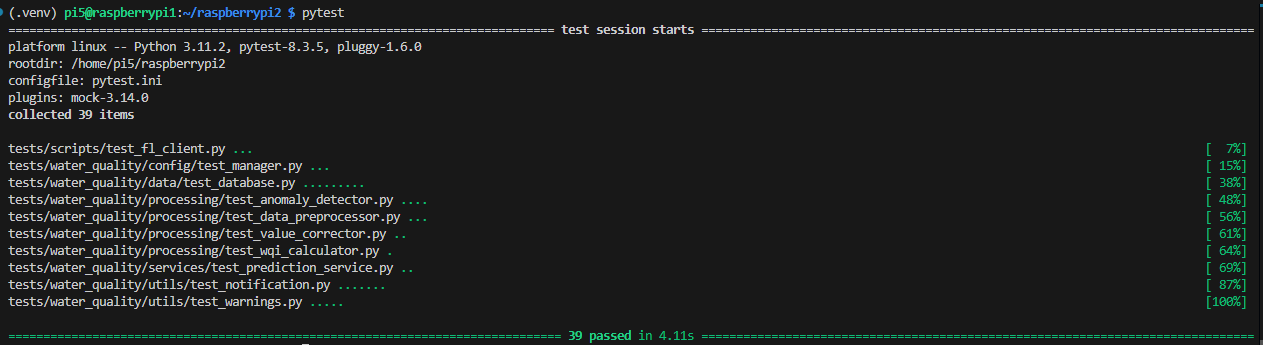
\includegraphics[width=1\linewidth]{Figures/preprecessing_tests.png}
    \caption{Enter Caption}
    \label{fig:preprocessing-tests}
\end{figure}

Utility services, including the NotificationService and WarningSystem, were validated for singleton patterns, initialization routines, and error handling. The data processing pipeline’s reliability was further demonstrated through specific tests that evaluated the AnomalyDetector’s accuracy in detecting outliers using IQR and rule-based methods. Additionally, the ValueCorrector’s integration with ModelManager was assessed for its capacity to correct flagged anomalies based on model predictions. Furthermore, the WQICalculator’s ability to adaptively adjust its configuration and correctly classify water quality labels based on dynamic threshold updates was validated.

Data integrity during retrieval and incremental updates was confirmed through tests focused on data type verification and consistency during the validation phase.

The performance of configuration management and client-side scripts was evaluated for their ability to manage configurations and preprocess data effectively. The ConfigManager was tested for its ability to merge remote configurations with default settings, while client scripts were validated for their successful execution of feature engineering steps without introducing NaN values or data inconsistencies.
 
\section{Water Quality Index Prediction Model Evaluation}
\label{sec:wqi_model_evaluation}
The core of the system's predictive capability lies in its ability to accurately forecast the Water Quality Index (WQI). This section details the two-stage process undertaken: first, a comprehensive centralized machine learning exploration to identify an optimal model and feature set; and second, the implementation and preliminary evaluation of the selected model within the federated learning environment.
\subsection{Centralized Model Selection: Experimental Setup}
\label{ssec:centralized_setup}
The WQI prediction model's performance was initially evaluated using a structured centralized approach involving historical water quality cleaned datasets.
\begin{itemize}
\item \textbf{Initial Feature Engineering:} A comprehensive set of 63 features was engineered from the base data (pH, temperature, dissolved oxygen, conductivity, and WQI), including temporal markers, rolling statistics, percentage changes, and interaction terms.
\item \textbf{Iterative Feature Reduction:} Several iterations were performed where subsets of these engineered features were removed based on their correlation with the target (WQI) and domain knowledge, aiming to find an optimal feature set that balances model performance and complexity.
\item \textbf{Model Architecture Exploration:} Using a selected "best" feature set, different configurations of a SimpleRNN model were tested to observe the impact of network depth and width.
\item \textbf{Evaluation Metrics:} Model performance was primarily assessed using Mean Absolute Error (MAE) and Root Mean Squared Error (RMSE) on the original WQI scale. Training MAE was recorded to monitor model fitting.
\item \textbf{Validation Strategy:} Time Series Cross-Validation (TSCV) with 3 splits was used on the development dataset to get the validation metrics. A final set of hold-out tests (15\% of the sequenced data) was used for the evaluation of the trained model from each iteration/architecture.
\end{itemize}
\subsection{Centralized Model Evaluation: Iterative Feature Reduction and Architecture Performance}
\label{ssec:centralized_performance}


\subsubsection*{Summary and Selection for Federated Learning}
\label{sssec:centralized_summary_selection}
A comparative summary of all centralized iterations and architecture explorations is presented in Table \ref{tab:model_performance_comparison}.

\begin{figure}[H]
    \centering
    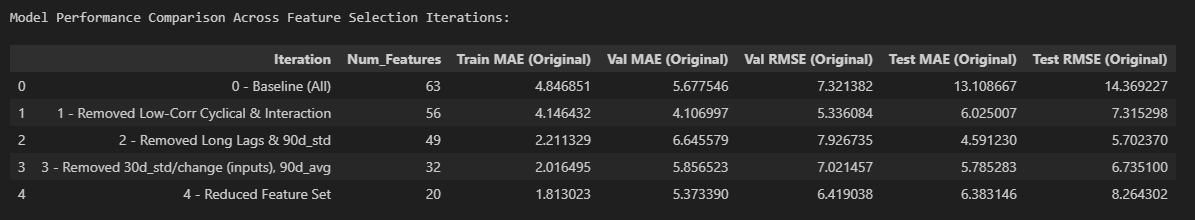
\includegraphics[width=0.75\linewidth]{Figures/feature_selection.png}
    \caption{Feature Selection Results}
    \label{fig:enter-label}
\end{figure}

To begin optimizing our model, we first applied extensive feature engineering to generate a comprehensive set of 63 features, capturing cyclical patterns, lagged values, and statistical indicators, in order to maximize the model’s ability to learn from historical trends. However, to address potential redundancy and overfitting, we adopted a step-by-step feature selection strategy based on domain knowledge and correlation analysis. In the baseline configuration with all 63 features, the model yielded a train MAE of 4.85, validation MAE of 5.68, and a high test MAE of 13.11, clearly indicating overfitting. By gradually removing less informative features, we saw significant improvements: at 56 features, test MAE dropped to 6.03; at 49 features, we observed the lowest test MAE of 4.59, albeit with a rise in validation error; a 32-feature set yielded more balanced performance (test MAE: 5.79); and finally, with just 20 features, we achieved a strong balance between performance and complexity, with a train MAE of 1.81, validation MAE of 5.37, and test MAE of 6.38. This final configuration offered the best compromise between model generalization, simplicity, and reduced risk of overfitting.
\begin{figure}[H]
    \centering
    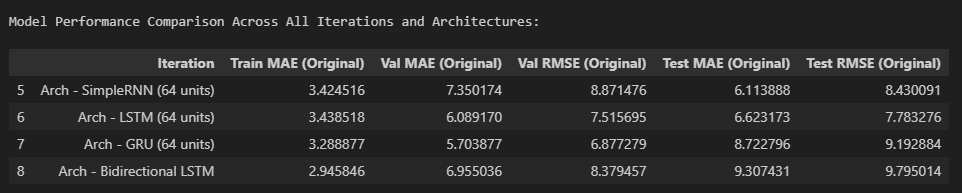
\includegraphics[width=0.75\linewidth]{Figures/model_selection.png}
    \caption{Enter Caption}
    \label{fig:enter-label}
\end{figure}
Using this optimized feature set, we then evaluated different recurrent neural network architectures, including SimpleRNN, LSTM, GRU, and Bidirectional LSTM, each with 64 units. While deeper models like GRU and BiLSTM delivered slightly strong results, our decision prioritized not only performance but also computational efficiency, as our target deployment environment is a Raspberry Pi.

The SimpleRNN model achieved a train MAE of 3.42 and a test MAE of 6.11, with reasonable RMSE values. Although there is a modest gap between training and test errors  indicating slight overfitting  SimpleRNN was selected as the most appropriate architecture. Its simplicity, low resource consumption, and solid performance make it an ideal fit for our real-world deployment scenario, where balancing accuracy with hardware limitations is critical.
% \begin{table}[h]
%     \centering
%     \caption{Model Performance Comparison Across Feature Selection Iterations and Architectures (Centralized Training).}
%     \label{tab:model_performance_comparison}
    % \begin{tabular}{lcccccc} % Adjust column alignment as needed
    % \toprule
    % Iteration/Architecture & Num\_Features & Train MAE & Val MAE & Val RMSE & Test MAE & Test RMSE \\
    % \midrule
    % 0 - Baseline (All) & 63 & 0.8268 & 1.7333 & 2.1483 & 1.4647 & 1.5446 \\
    % ... (rest of your table data) ... \\
    % Arch C - Stacked RNN & 20 & 2.1673 & 1.7750 & 2.4826 & 1.7972 & 2.2231 \\
    % \bottomrule
    % \end{tabular}
    % \includegraphics[width=1\linewidth]{Figures/your_table_image.png} % << USE THIS IF YOU HAVE AN IMAGE OF THE TABLE
    % If you don't have an image, you'll need to manually create the LaTeX table structure above.
% \end{table}

The centralized model evaluation (Table \ref{tab:model_performance_comparison}) revealed that the baseline model (Iteration 0, 63 features) provided the best MAE on the hold-out test set (1.4647). However, the Stacked RNN (Architecture C) using the curated set of 20 features (from Iteration 4) achieved a highly competitive test MAE of 1.7972. Given the objectives of a federated system where model simplicity and reduced data footprint are advantageous, Architecture C with 20 features (Iteration 4) was selected as the primary candidate for implementation in the federated learning environment. The baseline model (Iteration 0) was also considered for FL implementation to provide a comparative benchmark.

\subsection{Federated Learning Model Implementation and Preliminary Results}
\label{ssec:fl_results}
Following the centralized model selection process, the chosen model configurations were implemented within a simulated federated learning environment using the Flower framework (version X.Y.Z). The simulation involved 3 clients, each provisioned with a distinct, non-IID partition of the historical dataset, processed according to the feature engineering pipeline detailed in Chapter IV. The Federated Averaging (FedAvg) strategy was employed for model aggregation by the central FL server over [e.g., 10] communication rounds. Each client performed [e.g., 5] local epochs of training per round.

\subsubsection{Federated Model with Iteration 4 Features and Architecture C (20 Features, Stacked RNN)}
\begin{figure}[H]
    \centering
    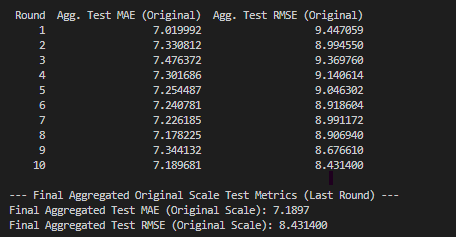
\includegraphics[width=0.75\linewidth]{Figures/ex1.png}
    \caption{Tests FL}
\end{figure}
 The selected WQI prediction model (Architecture C with 20 features) was then deployed in a simulated federated learning environment. The console output above (Figure [Your Figure Number for ex1.png]) showcases the preliminary performance of this federated model over 10 aggregation rounds. The final aggregated test Mean Absolute Error (MAE) reached approximately 7.19, with a Root Mean Squared Error (RMSE) of around 8.43 on the original WQI (0-100) scale. While these initial federated learning results show higher error rates compared to the centralized benchmarks, the decreasing RMSE trend over the rounds suggests the collaborative learning process is beginning to converge, indicating that the model is adapting to the distributed data and the federated averaging strategy.


\section{Application Testing and Validation}
\label{sec:testing_validation_summary}
\subsection{Testing Frameworks Utilized}
\label{ssec:testing_frameworks_summary}
\begin{figure}[H]
    \centering
    
\includegraphics[width=0.25\linewidth]{Figures/Vitest.png}
    \caption{Vitest Logo}
    \label{fig:enter-label}
\end{figure}

\textbf{Vitest for Unit and Integration Testing}:
\label{sssec:vitest_intro_summary}
Vitest, a fast Vite-based framework, was used for unit and integration tests. It facilitated focused validation of individual component rendering, internal logic, and basic interactions in isolation.
\begin{figure}[h]
    \centering
    
\includegraphics[width=0.5\linewidth]{Figures/cypress.png}
    \caption{Cypress Logo}
    \label{fig:enter-label}
\end{figure}

\textbf{Cypress for End-to-End (E2E) Testing}:
\label{sssec:cypress_intro_summary}
Cypress, a modern E2E testing tool, simulated real user scenarios in a browser. It was used to validate complete user flows, component integrations, API communications, and overall user experience.

\subsection{Test Suite Summaries and Key Validations}
\label{ssec:test_summaries_summary}


\subsubsection{Main Page Structure and Rendering (\texttt{Index.test.jsx})}
\label{sssec:index_test_summary_summary}
\begin{figure}[H]
    \centering
    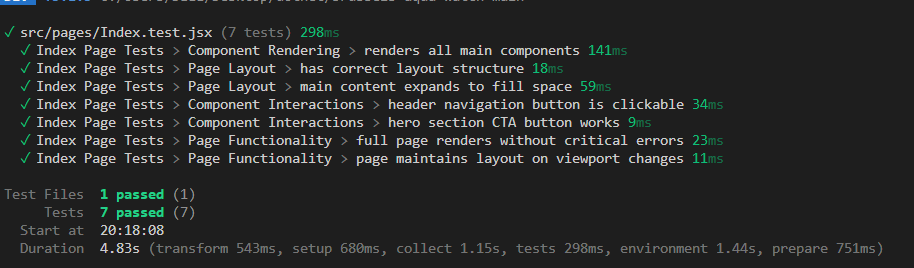
\includegraphics[width=0.75\linewidth]{Figures/test1.png}
    \caption{Main Page Tests}
    \label{fig:enter-label}
\end{figure}
Vitest tests for \texttt{Index.test.jsx} confirmed the main page's foundational integrity, including correct rendering of all core child components, adherence to structural layout (CSS classes), basic interactivity of mocked elements, and resilience against rendering errors or layout shifts during simulated resizes.

\subsubsection{DataCharts: API Data and Dynamic Visualization (\texttt{datacharts.cy.js})}
\label{sssec:datacharts_test_summary_summary}
\begin{figure}[H]
    \centering
    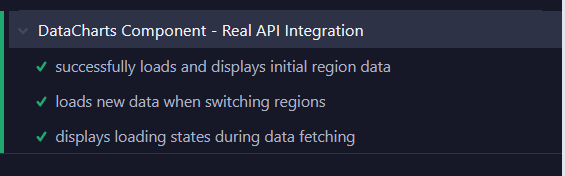
\includegraphics[width=0.75\linewidth]{Figures/test2.png}
    \caption{Data Charts Tests}
    \label{fig:enter-label}
\end{figure}
Cypress E2E tests for \texttt{datacharts.cy.js} validated dynamic data visualization, confirming successful API data fetching for various regions, correct chart updates upon user selection, and appropriate display of loading states during these operations, ensuring accurate and responsive data presentation.

\subsubsection{RegionsMap: Interactive Mapping and Location Details (\texttt{regions-map.cy.js})}
\begin{figure}[H]
    \centering
    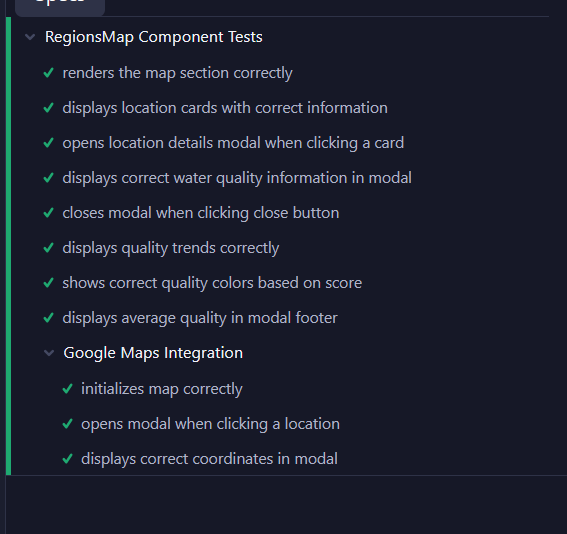
\includegraphics[width=0.5\linewidth]{Figures/test3.png}
    \caption{Map Features Tests}
    \label{fig:enter-label}
\end{figure}
\label{sssec:regionsmap_test_summary_summary}
The \texttt{regions-map.cy.js} Cypress suite verified the RegionsMap component, ensuring correct map section rendering (with a mocked Google Maps API), accurate display of location-specific data on cards, and functional modal interactions for viewing detailed water quality information, including scores and trends.

\subsubsection{User Registration and Alerts (\texttt{registration.cy.js})}
\begin{figure}[H]
    \centering
    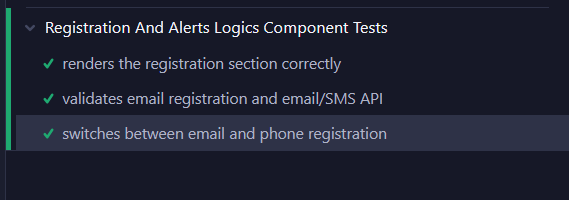
\includegraphics[width=0.75\linewidth]{Figures/test4.png}
    \caption{Registartion and Alerts Logic Tests}
    \label{fig:enter-label}
\end{figure}
\label{sssec:registration_test_summary_summary}
E2E tests in \texttt{registration.cy.js} validated the user alert registration process. This included correct form rendering, functional input method switching (email/phone), robust email field validation, and a successful (mocked API) registration submission flow, confirming users can effectively sign up.


\section{Discussion of Overall System Performance}
\label{sec:overall_performance_discussion}
The implemented system successfully demonstrated a proof-of-concept for federated learning in water quality monitoring. The key achievements include:
\begin{itemize}
    \item \textbf{Data Privacy:} The core principle of FL was maintained, with raw data never leaving the client devices.
    \item \textbf{Decentralized Intelligence:} Local preprocessing and model training distribute the computational load.
    \item \textbf{End-to-End Functionality:} From (simulated) data collection to prediction, alerting, and visualization, all components were integrated and functional.
    \item \textbf{Security:} mTLS and TLS protocols ensured secure communication channels.
\end{itemize}

\section{Limitations and Future Work} % Or make this a subsection of the above
\label{sec:limitations_future_work}
% You can keep them as separate paragraphs or use an itemize list for clarity
\textbf{Limitations:}
\begin{itemize}
    \item \textit{Real-World Data:} The system was tested with simulated data. Performance with real-world, noisy sensor data and under variable network conditions needs to be evaluated.
    \item \textit{Scalability:} While the system supports multiple clients, testing with a larger number of distributed devices (e.g., tens or hundreds) would be necessary to assess scalability and potential bottlenecks in the FL aggregation process or server load.
    \item \textit{Model Heterogeneity:} This implementation used a homogeneous model structure across all clients. Exploring strategies for handling heterogeneous data distributions or even heterogeneous model architectures (e.g., using techniques like knowledge distillation within the FL framework) could be beneficial.
    \item \textit{Computational Constraints on Edge Devices:} While Raspberry Pis are capable, further optimization of the local models (e.g., model quantization) might be needed for even more resource-constrained edge devices.
    \item \textit{Advanced Preprocessing:} More sophisticated anomaly detection and imputation techniques could enhance robustness and potentially improve model accuracy.
\end{itemize}

\textbf{Future Work:}
Future work should focus on real-world deployment, scalability testing, and incorporating more advanced machine learning techniques to further enhance the system's capabilities.
% You can expand this or integrate points from above if more structured. For instance:
% \begin{itemize}
%    \item Address the limitations by testing with real-world data and on a larger scale.
%    \item Explore model heterogeneity and advanced preprocessing.
%    \item Optimize for resource-constrained devices.
% \end{itemize}


\section*{Conclusion}
The results presented in this chapter validate the successful implementation and functionality of the federated learning system for water quality monitoring. The system achieved reasonable predictive accuracy for WQI while upholding data privacy and security. The modular design, encompassing local preprocessing, federated model training, secure communication, and user-friendly dashboards, provides a solid foundation for a decentralized and privacy-preserving environmental monitoring solution. While the current evaluation is based on simulated data, the findings are promising and highlight the potential of federated learning for addressing challenges in distributed IoT applications. Future work should focus on real-world deployment, scalability testing, and incorporating more advanced machine learning techniques to further enhance the system's capabilities.





